\documentclass[border=4pt]{standalone}
\usepackage{amsmath,amssymb,tikz}
\usetikzlibrary{arrows.meta}
\definecolor{figB}{RGB}{31,90,166}\definecolor{figR}{RGB}{176,48,48}\definecolor{figG}{RGB}{60,130,60}
\begin{document}
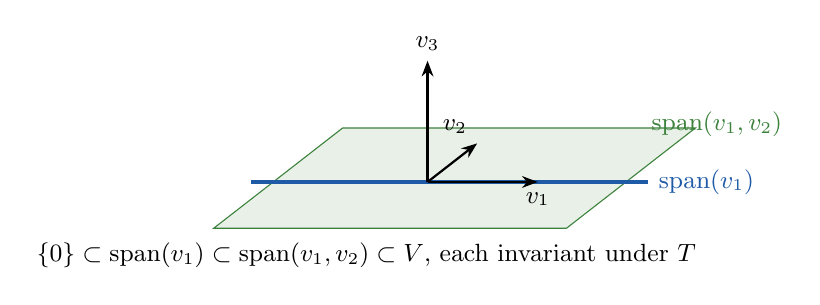
\begin{tikzpicture}[scale=1.4,>={Stealth[length=2mm]},x={(1cm,0cm)},y={(0.45cm,0.35cm)},z={(0cm,1cm)}]
\fill[figG!12] (-1.4,-1.2,0)--(1.8,-1.2,0)--(1.8,1.4,0)--(-1.4,1.4,0)--cycle;
\draw[figG] (-1.4,-1.2,0)--(1.8,-1.2,0)--(1.8,1.4,0)--(-1.4,1.4,0)--cycle;
\node[figG,font=\small] at (1.95,1.5,0) {$\operatorname{span}(v_1,v_2)$};
\draw[very thick,figB] (-1.6,0,0)--(2.0,0,0) node[right,font=\small]{$\operatorname{span}(v_1)$};
\draw[->,thick] (0,0,0)--(1,0,0) node[below,font=\small]{$v_1$};
\draw[->,thick] (0,0,0)--(0,1,0) node[above left,font=\small]{$v_2$};
\draw[->,thick] (0,0,0)--(0,0,1.1) node[above,font=\small]{$v_3$};
\node[font=\small,align=left] at (0.3,-1.9,0) {$\{0\}\subset\operatorname{span}(v_1)\subset\operatorname{span}(v_1,v_2)\subset V$, each invariant under $T$};
\end{tikzpicture}
\end{document}
